\documentclass{assignment}
\usepackage[pdftex]{graphicx}
\usepackage{xcolor}
\definecolor{LightGray}{gray}{0.95}
\usepackage{fancyvrb, minted}
\usepackage[letterpaper, margin = 2.5cm]{geometry}
\usepackage[T1]{fontenc}
\usepackage{amsmath, amsfonts, amssymb}
\usepackage{hyperref, url} 
\usepackage{fancyhdr}
\usepackage{enumitem}
\usepackage{listings}

\newcommand{\R}{\mathbb{R}}

\student{Aren Ashlock}   
\semester{Spring 2024}                         
\date{March ??, 2024}  

\courselabel{COM S 474/574} 
\exercisesheet{HW4}{Kernel Method}

\school{Department of Computer Science}
\university{Iowa State University}

\begin{document}
\begin{problem}

%----------------------------------------- 1 DONE -----------------------------------------

\section{Clustering, SVM, \& Kernel Method}

\begin{enumerate}

    \item Consider the Lloyed's algorithm for K-means, given the following clusters:

    \begin{itemize}
        \item $C_1 = \{(0,0), (10,10), (100,100)\}$
        \item $C_2 = \{(1,1), (0,5), (-3,4)\}$
        \item $C_3 = \{(-1,1), (0,-10), (30,-4)\}$
    \end{itemize}
    
    \begin{enumerate}[label=(\alph*)]

%---------------------------------------- 1A DONE -----------------------------------------
    
        \item Formulate the K-means problem as an optimization problem using the given data (of 9 points).

        \color{blue}\textbf{Answer:} $\min \sum_{k=1}^3 \sum_{x \in C_k} ||x - c_k||^2$ \color{black}

%------------------------------------------------------------------------------------------

%---------------------------------------- 1B DONE -----------------------------------------
        
        \item What are your updated clusters after one step of iteration? Please explain your steps to derive your answer.

        \color{blue}\textbf{Answer:} Using the initially defined clusters to find the centroids (the average of the points in the cluster), I took each point in the data and calculated the minimal cost from each centroid (using the minimization equation above), then I assigned the point to that cluster associated with the centroid. For example, $(0,0)$ belongs in $C_2$ because $((0-\frac{-2}{3})^2 + (0-\frac{10}{3})^2)$ is the minimal cost.\\
        $C_1 = \{(100,100)\}$\\
        $C_2 = \{(0,0), (10,10), (1,1), (0,5), (-3,4), (-1,1)\}$\\
        $C_3 = \{(0,-10), (30,-4)\}$
        \color{black}

%------------------------------------------------------------------------------------------

%---------------------------------------- 1C DONE -----------------------------------------
        
        \item Consider using $\ell_1$-norm as the distance (cost) measure.

        \begin{enumerate}[label=\roman*.]

%---------------------------------------- 1Ci DONE ----------------------------------------
        
            \item What are your updated clusters after one step of iteration? Please explain your steps to derive your answer.

            \color{blue}\textbf{Answer:} Using the initially defined clusters to find the centroids (the average of the points in the cluster), I took each point in the data and calculated the minimal cost from each centroid by summing the absolute value distance from the centroid for each coordinate, then I assigned the point to that cluster associated with the centroid. For example, $(0,0)$ belongs in $C_2$ because $(|0-\frac{-2}{3}| + |0-\frac{10}{3}|)^2$ is the minimal cost.\\
            $C_1 = \{(100,100)\}$\\
            $C_2 = \{(0,0), (1,1), (0,5), (-3,4), (-1,1), (0,-10)\}$\\
            $C_3 = \{(10,10), (30,-4)\}$ \color{black}

%------------------------------------------------------------------------------------------

%--------------------------------------- 1Cii DONE ----------------------------------------
        
            \item In what situations would you prefer to use this cost instead of the standard K-means clustering?

            \color{blue}\textbf{Answer:} You would want to utilize this cost instead of the standard K-means clustering when there are potential outliers in the data set. By having a higher p-norm, the distance range for the centroid includes more points, which could potentially include outliers that skew the clustering. \color{black}

%------------------------------------------------------------------------------------------

        \end{enumerate}

%------------------------------------------------------------------------------------------

%---------------------------------------- 1D DONE -----------------------------------------
        
        \item Use \texttt{\textbf{sklearn.cluster.KMeans}} to cluster the data set of the above 9 points. Set $K = 2$ (two clusters). Feel free to play with the arguments. Show me your code, and plot your clustered outcome (use different colors to differentiate the clusters).

        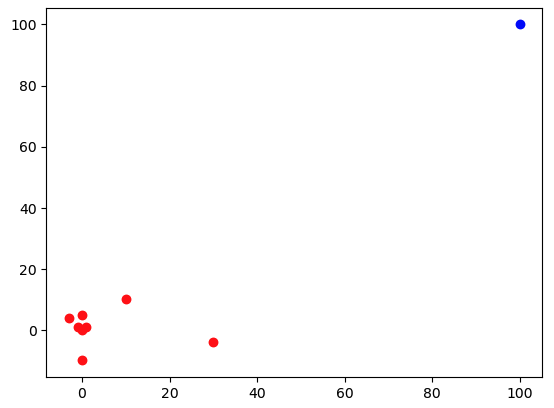
\includegraphics[scale=.5]{474-HW4-Q1.png}

        \color{blue}\textbf{Code:}
        \begin{lstlisting}
from sklearn.cluster import KMeans
import numpy as np

X = np.array([[0,0],[10,10],[100,100],[1,1],[0,5],[-3,4],[-1,1],[0,-10],[30,-4]])
kmeans = KMeans(n_clusters=2, n_init="auto").fit(X)
clusters = kmeans.fit_predict(X)

cluster0 = X[clusters==0]
cluster1 = X[clusters==1]
 
plt.scatter(cluster0[:,0] , cluster0[:,1] , color = 'red')
plt.scatter(cluster1[:,0] , cluster1[:,1] , color = 'blue')
plt.show()
        \end{lstlisting}
        \color{black}

%------------------------------------------------------------------------------------------

    \end{enumerate}

%----------------------------------------- 2 DONE -----------------------------------------

    \item Consider the following two clusters:
    
    \begin{itemize}
        \item $C_1 = \{(x,y) | y \geq x^2 + 2, x \in \R\}$
        \item $C_2 = \{(x,y) | y \leq x^2 - 2, x \in \R\}$
    \end{itemize}

    Are the two clusters linearly separable? What kernel trick can you apply here (specifically what feature transform $\phi : \R^2 \rightarrow \mathcal{F}$) to make them linearly separable? Is this kernel trick unique?

    \color{blue}\textbf{Answer:} In their original form, the two clusers are \textbf{NOT} linearly separable. We can utilize the polynomial kernel trick, which has $\phi(x) = \begin{bmatrix}x_1^2 & \sqrt{2}x_1x_2 & x_2^2\end{bmatrix}^T$ and $\phi(x) = \begin{bmatrix}y_1^2 & \sqrt{2}y_1y_2 & y_2^2\end{bmatrix}^T$. \textbf{NO}, this kernel trick is not unique. \color{black}

%------------------------------------------------------------------------------------------

%----------------------------------------- 3 DONE -----------------------------------------

    \item Recall the proof of convergence of Gradient Descent with $L$-smooth function. Try to use a similar idea to prove the convergence of Lloyed's algorithm for K-means.

    \color{blue}\textbf{Answer:} The formulation of Lloyed's algorithm is based on minimizing $J(C)$. In each iteration of the algorithm, the centroid(s) adjust their position in order to minimize the distance from it to all the points in the cluster it belongs to. Therefore, as each iteration occurs, $J(C)$ either gets smaller or doesn't change. This results in a monotomically decreasing function, which shows that Lloyed's algorithm converges. \color{black}

%------------------------------------------------------------------------------------------

%----------------------------------------- 4 DONE -----------------------------------------

    \item Consider the following data set with features $x_i \in \R^2, \forall i$ and binary class labels $y_i \in \{1, -1\}, \forall i, X = \{(0,2), (0.4,1), (0.6,1), (1,0)\}, y = \{-1, -1, 1, 1\}$:
    
    \begin{enumerate}[label=(\alph*)]

%---------------------------------------- 4A DONE -----------------------------------------
    
        \item Using a scatter plot of the data, devise a linear classifier of the form

        \begin{equation}
            \hat{y} = \begin{cases}
                1 &  \text{if } b + w^Tx \geq 0\\
                -1 & \text{if } b + w^Tx < 0
                \tag*{(1-1)}
            \end{cases} 
        \end{equation}

        that separates the two classes. What is your selected $b$ and $w$? Is the selection unique?

        \color{blue}\textbf{Answer:} $w = \begin{bmatrix}3 & 1\end{bmatrix}^T, b = -2.5$ \textbf{NO}, this selection is not unique. \color{black}

%------------------------------------------------------------------------------------------

%---------------------------------------- 4B DONE -----------------------------------------
        
        \item Compute the distance of the closest sample to the classifier boundary. Show me your equation and the sample(s) that are the closest.

        \color{blue}\textbf{Answer:} $\frac{w^T x_i + b}{\sqrt{10}} \rightarrow \frac{3(0) + 1(2) - 2.5}{\sqrt{10}} \approx -0.158, \frac{3(0.4) + 1(1) - 2.5}{\sqrt{10}} \approx -0.095, \frac{3(0.6) + 1(1) - 2.5}{\sqrt{10}} \approx 0.095, \frac{3(1) + 1(0) - 2.5}{\sqrt{10}} \approx 0.158$\\
        The closest points are $(0.4,1)$ and $(0.6,1)$ with a distance of $0.095$. \color{black}

%------------------------------------------------------------------------------------------

%---------------------------------------- 4C DONE -----------------------------------------
        
        \item Scale your classifier so that $y_i(b + w^Tx_i) = 1$ for the closest sample(s) $i$ and report the new $b$ and $w$. Is $\frac{1}{||w||}$ the same with the minimum distance from question 4(b)?

        \color{blue}\textbf{Answer:} $1(-(s)2.5 + (s)(3(0.6) + 1(1))) = 1 \rightarrow s = \frac{1}{-2.5 + 3(0.6) + 1(1)} \rightarrow s = 10/3$\\
        $w = \begin{bmatrix}10 & 10/3\end{bmatrix}^T, b = -25/3$\\
        $\frac{1}{||w||} = \frac{1}{\sqrt{(10)^2 + (10/3)^2}} \approx 0.095 \rightarrow$ \textbf{YES}, it is the same as the minimum distance \color{black}

%------------------------------------------------------------------------------------------

    \end{enumerate}

%----------------------------------------- 5 DONE -----------------------------------------

    \item Create a data set yourself with $X \subset \R^n$ and the classified labels $y \in \{-1, 1\}$.
    
    \begin{enumerate}[label=(\alph*)]

%---------------------------------------- 5A DONE -----------------------------------------
    
        \item Give the scatter plot of the data you created, use colors to differentiate the different labels.

        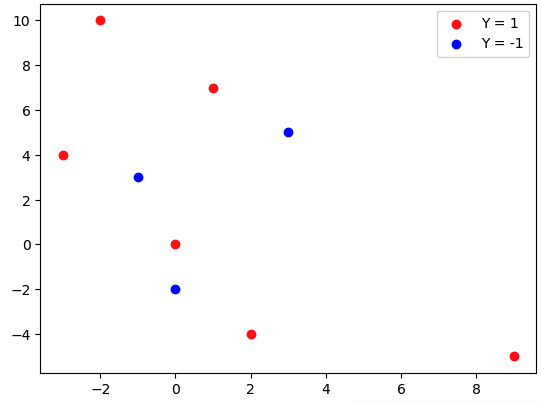
\includegraphics[scale=.4]{474-HW4-Q5-a.png}

%------------------------------------------------------------------------------------------

%---------------------------------------- 5B DONE -----------------------------------------
        
        \item Use the SVC tools from \texttt{sklearn} to create a \textbf{linear} classifier for your data set and show it on the plot (note \texttt{sklearn} has at least two ways to implement a linear SVC: \texttt{svm.LinearSVC} and \texttt{svm.SVC} with the argument kernel set to ''linear", \texttt{svm.LinearSVC} is generally faster).

        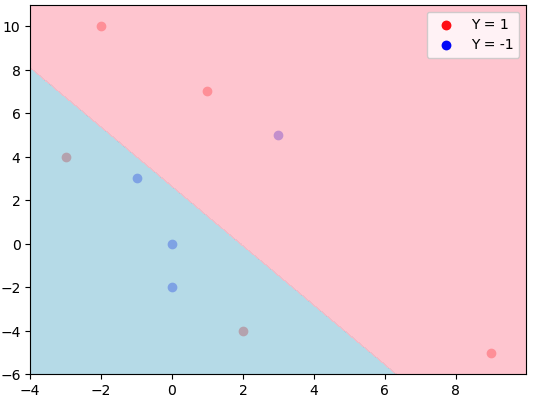
\includegraphics[scale=.4]{474-HW4-Q5-b.png}

%------------------------------------------------------------------------------------------

%---------------------------------------- 5C DONE -----------------------------------------
        
        \item Recall the logistic regression introduced in the previous lecture, use\\ 
        \texttt{sklearn.linear\_model.LogisticRegression} to create another linear classifier for your data set. Show it on the plot, and compare it with the SVC-based solution.

        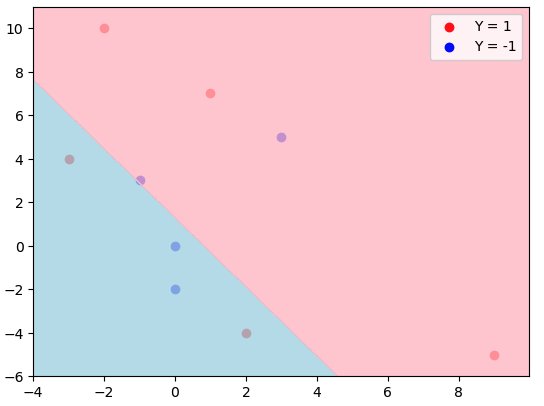
\includegraphics[scale=.4]{474-HW4-Q5-c.png}\\
        \color{blue}\textbf{Comparison:} The linear classifiers are extremely similar with just slight variations in the slope and intercept of the line. The LogisticRegression seems to fit less optimally since there is one more point that is classified incorrectly compared to SVC(linear). \color{black}

%------------------------------------------------------------------------------------------

    \end{enumerate}
\end{enumerate}
\end{problem}
\end{document}